\chapter{Results and Analysis}\label{chap:results}

\section{TLS connections}
% Begin with the benchmark done by Bastien on the raw number of verif/s with openssl.

This benchmark is done only with OpenVPN.
Since there is no standard support for those operation in the kernel yet, it would not have made sense to use IPSec, since it would have had to fallback to OpenSSL, then following the same path as OpenVPN do.
As soon as the public key operations can be plugged into the crypto API, this use case should however be tested immediatly.


\section{Response time -- latency}
After the establishement of a connection.

\subsection{OpenVPN}

\begin{figure}[ht]
%%%%%%%%%%%%%%%%%%%%%%%%%%%%%%%%%%%%%%%%%%%%%%%%%%%%%%%%%%
% Ping GCM
%%%%%%%%%%%%%%%%%%%%%%%%%%%%%%%%%%%%%%%%%%%%%%%%%%%%%%%%%%
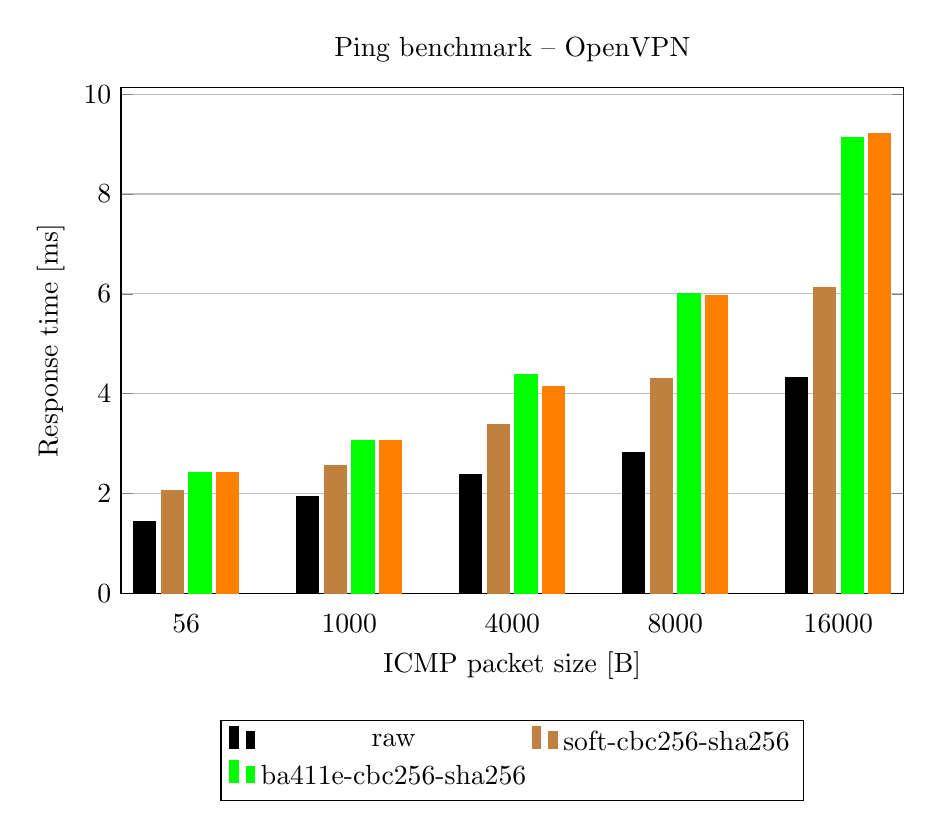
\begin{tikzpicture}
\begin{axis}[
        title = {Ping benchmark -- OpenVPN},
        width  = 0.95*\textwidth,
        height = 8cm,
        major x tick style = transparent,
        ybar,
        bar width=8pt,
        ymajorgrids = true,
        ylabel = {Response time [ms]},
        xlabel = {ICMP packet size [B]},
        ymin=0,
        symbolic x coords={56, 1000, 4000, 8000, 16000},
        xtick = data,
        scaled y ticks = false,%Disable the *10^4 exponent applied to all y axis markings.
        legend style={at={(0.5,-0.25)}, anchor=north,legend columns=2},
        enlarge x limits=0.1,
    ]
% I would have prefered to have "\addplot[marks only]", but they overlap if they have the same x coordinate,
% not like bars that automatically shift.
\addplot[style={black, fill=black}]
    coordinates {
        (56, 1.444)
        (1000, 1.929)
        (4000, 2.376)
        (8000, 2.811)
        (16000, 4.322)
    };
    \label{raw}

\addplot[style={brown, fill=brown}]
    coordinates {
        (56, 2.066)
        (1000, 2.561)
        (4000, 3.373)
        (8000, 4.293)
        (16000, 6.117)
    };
    \label{none-none}

\addplot[style={green, fill=green}]
    coordinates {
        (56, 2.415)
        (1000, 3.061)
        (4000, 4.376)
        (8000, 5.997)
        (16000, 9.135)
    };
    \label{soft-cbc256-sha256}

\addplot[style={orange, fill=orange}]
    coordinates {
        (56, 2.416)
        (1000, 3.052)
        (4000, 4.140)
        (8000, 5.963)
        (16000, 9.207)
    };
    \label{ba411e-cbc256-sha256}

\legend{raw, soft-cbc256-sha256, ba411e-cbc256-sha256}
\end{axis}
\end{tikzpicture}
% Here, I could show the gcm128, which show better performances with the BA411e, but I would be weird to compare it with aes256cbc.
% I need another graph with a CPu usage comparison to show that even if the perf are the same for soft/hard with aes256gcm, the hard loads less the CPU (I hope so, at least).
\caption{Ping min/avg/max response time}{for different packet sizes using OpenVPN}
\label{fig:ping-benchmark-openvpn}
\end{figure}

\subsection{IPSec}

\begin{figure}[ht]
%%%%%%%%%%%%%%%%%%%%%%%%%%%%%%%%%%%%%%%%%%%%%%%%%%%%%%%%%%
% Ping GCM
%%%%%%%%%%%%%%%%%%%%%%%%%%%%%%%%%%%%%%%%%%%%%%%%%%%%%%%%%%
\begin{tikzpicture}
\begin{axis}[
        title = {Ping benchmark -- IPsec},
        width  = \textwidth,
        height = 8cm,
        major x tick style = transparent,
        ybar,
        bar width=8pt,
        ymajorgrids = true,
        ylabel = {Response time [ms]},
        xlabel = {ICMP packet size [B]},
        ymin=0, ymax=10,
        symbolic x coords={56, 1000, 8000, 16000},
        xtick = data,
        scaled y ticks = false,%Disable the *10^4 exponent applied to all y axis markings.
        legend style={at={(0.5,-0.25)}, anchor=north,legend columns=3},
        enlarge x limits=0.15,
    ]
% I would have prefered to have "\addplot[marks only]", but they overlap if they have the same x coordinate,
% not like bars that automatically shift.
\addplot[style={black, fill=black}]
    coordinates {
        (56, 1.444)
        (1000, 1.929)
        (8000, 2.811)
        (16000, 4.322)
    };
    \label{raw}

\addplot[style={NavyBlue, fill=NavyBlue}]
    coordinates {
        (56, 1.545)
        (1000, 2.045)
        (8000, 2.997)
        (16000, 4.703)
    };
    \label{none-none}

\addplot[style={OliveGreen, fill=OliveGreen},postaction={pattern=north east lines}]
    coordinates {
        (56, 1.581)
        (1000, 2.134)
        (8000, 3.910)
        (16000, 6.426)

    };
    \label{soft-cbc256-none}

\addplot[style={BrickRed, fill=BrickRed},postaction={pattern=north east lines}]
    coordinates {
        (56, 1.639)
        (1000, 2.080)
        (8000, 3.445)
        (16000, 5.345)
    };
    \label{ba411e-cbc256-none}

\addplot[style={OliveGreen, fill=OliveGreen}]
    coordinates {
        (56, 1.645)
        (1000, 2.322)
        (8000, 4.762)
        (16000, 7.975)

    };
    \label{soft-cbc256-sha256}

\addplot[style={BrickRed, fill=BrickRed}]
    coordinates {
        (56, 1.635)
        (1000, 2.246)
        (8000, 4.170)
        (16000, 6.929)
    };
    \label{ba411e-cbc256-sha256}

\addplot[style={OliveGreen, fill=OliveGreen},postaction={pattern=north west lines}]
    coordinates {
        (56, 1.651)
        (1000, 2.388)
        (8000, 5.383)
        (16000, 9.241)
    };
    \label{soft-gcm256}

\addplot[style={BrickRed, fill=BrickRed},postaction={pattern=north west lines}]
    coordinates {
        (56, 1.764)
        (1000, 2.286)
        (8000, 0)
        (16000, 0)
    };
    \label{ba411e-gcm256}

\legend{raw, none-none, soft-cbc256-none, ba411e-cbc256-none, soft-cbc256-sha256, ba411e-cbc256-sha256, soft-gcm256, ba411e-gcm256}
\end{axis}
\end{tikzpicture}
% Here, I could show the gcm256, which show better performances with the BA411e, but I would be weird to compare it with aes256cbc.
% I need another graph with a CPu usage comparison to show that even if the perf are the same for soft/hard with aes256gcm, the hard loads less the CPU (I hope so, at least).
\caption{Ping min/avg/max response time}{for different packet sizes using IPsec. For each packet size, 1000 requests were flooded to the board, that is \textit{"outputs packets as fast as they come back or one hundred times per second, whichever is more"}, according to the \texttt{ping} command manual.} %TODO move the end of the caption to the "test protocol" chapter.
\label{fig:ping-benchmark-ipsec}
\end{figure}


\section{File transfer}
%FTP over openvpn and IPSec

%OpenSSH: 	- normal transfer: shows perf difference
%			- capped to software max: show CPU offload

\subsection{openSSH}

\begin{figure}[ht]
\begin{tikzpicture}

%%%%%%%%%%%%%%%%%%%%%%%%
% CPU in the background
%%%%%%%%%%%%%%%%%%%%%%%%
\begin{axis}[
        width  = 0.95*\textwidth,
        height = 8cm,
        major x tick style = transparent,
        ybar=2pt,%space between the bars
        bar width=16pt,
        enlarge x limits={abs=1},
        ylabel = {CPU\#0 usage},
        hide x axis,
        axis y line*=right,
        ymin=0, ymax=100,
        symbolic x coords={none:none, aes256cbc:none, aes256cbc:sha256},
        xtick = data,
        scaled y ticks = false,%Disable the *10^4 exponent applied to all y axis markings.
        legend style={at={(0.5,-0.15)}, anchor=north,legend columns=4},
        enlarge x limits=0.1,
    ]

\addplot[style={black,fill=LimeGreen,postaction={pattern=north east lines},mark=none}]
    coordinates {
        (none:none, 0)
        (aes256cbc:none, 96.26)
        (aes256cbc:sha256, 89.29)
    };
    \label{software}

\addplot[style={black,fill=RedOrange,postaction={pattern=north east lines},mark=none}]
    coordinates {
        (none:none, 0)
        (aes256cbc:none, 46.01)
        (aes256cbc:sha256, 68.19)
    };
    \label{ba411e}

\addplot[style={black,fill=gray,postaction={pattern=north east lines},mark=none}]
    coordinates {
        (none:none, 7.16)
        (aes256cbc:none, 0)
        (aes256cbc:sha256, 0)
    };
    \label{out-of-tunnel}%"oot" for "out of tunnel"
\legend{software, ba411e, out-of-tunnel}
\end{axis}

%%%%%%%%%%%%%%%%%%%%%%%%
% throughput
%%%%%%%%%%%%%%%%%%%%%%%%
\begin{axis}[
        title = {File transfer over an SSH tunnel},
        width  = 0.95*\textwidth,
        height = 8cm,
        major x tick style = transparent,
        ybar=10pt,
        bar width=8pt,
        enlarge x limits={abs=1},
        ymajorgrids = true,
        ylabel = {Throughtput [MB/s]},
        xlabel = {},
        ymin=0, ymax=12,
        symbolic x coords={oot, none:none, aes256cbc:none, aes256cbc:sha256},
        xtick = data,
        scaled y ticks = false,%Disable the *10^4 exponent applied to all y axis markings.
        legend style={at={(0.5,-0.25)}, anchor=north,legend columns=2},
        enlarge x limits=0.1,
    ]

\addplot[style={black,fill=ForestGreen,mark=none}]
    coordinates {
        (none:none, 0)
        (aes256cbc:none, 10.89)
        (aes256cbc:sha256, 8.19)
    };
    \label{soft-tp}

\addplot[style={black,fill=BrickRed,mark=none}]
    coordinates {
        (none:none, 0)
        (aes256cbc:none, 10.67)
        (aes256cbc:sha256, 10.39)
    };
    \label{ba411e-tp}

\addplot[style={black,fill=black,mark=none}]
    coordinates {
        (none:none, 11.39)
        (aes256cbc:none, 0)
        (aes256cbc:sha256, 0)
    };
    \label{oot-tp}%"tp" for "throughput"
\legend{}
\end{axis}

\end{tikzpicture}
\caption{file transfer over an SSH tunnel. The background stripped bars are the CPU usage.}{}
\label{fig:openssh-bench}
\end{figure}

\subsection{OpenVPN}

\begin{figure}[ht]
\begin{tikzpicture}

%%%%%%%%%%%%%%%%%%%%%%%%
% CPU in the background
%%%%%%%%%%%%%%%%%%%%%%%%
\begin{axis}[
        width  = 0.95*\textwidth,
        height = 8cm,
        major x tick style = transparent,
        ybar=2pt,%space between the bars
        bar width=16pt,
        enlarge x limits={abs=1},
        ylabel = {CPU\#0 usage},
        hide x axis,
        axis y line*=right,
        ymin=0, ymax=100,
        symbolic x coords={none:none, aes256cbc:none, aes256cbc:sha256},
        xtick = data,
        scaled y ticks = false,%Disable the *10^4 exponent applied to all y axis markings.
        legend style={at={(0.5,-0.15)}, anchor=north,legend columns=4},
        enlarge x limits=0.1,
    ]

\addplot[style={black,fill=LimeGreen,postaction={pattern=north east lines},mark=none}]
    coordinates {
        (none:none, 0)
        (aes256cbc:none, 76.60)
        (aes256cbc:sha256, 76.03)
    };
    \label{software}

\addplot[style={black,fill=RedOrange,postaction={pattern=north east lines},mark=none}]
    coordinates {
        (none:none, 0)
        (aes256cbc:none, 83.74)
        (aes256cbc:sha256, 80.89)
    };
    \label{ba411e}

\addplot[style={black,fill=gray,postaction={pattern=north east lines},mark=none}]
    coordinates {
        (none:none, 7.16)
        (aes256cbc:none, 0)
        (aes256cbc:sha256, 0)
    };
    \label{out-of-tunnel}%"oot" for "out of tunnel"

\addplot[style={black,fill=brown,postaction={pattern=north east lines},mark=none}]
    coordinates {
        (none:none, 42.60)
        (aes256cbc:none, 0)
        (aes256cbc:sha256, 0)
    };
    \label{inside tunnel}%"it" for "in tunnel"
\legend{software, ba411e, out-of-tunnel, inside tunnel}
\end{axis}

%%%%%%%%%%%%%%%%%%%%%%%%
% throughput
%%%%%%%%%%%%%%%%%%%%%%%%
\begin{axis}[
        title = {FTP transfer inside OpenVPN tunnel},
        width  = 0.95*\textwidth,
        height = 8cm,
        major x tick style = transparent,
        ybar=10pt,
        bar width=8pt,
        enlarge x limits={abs=1},
        ymajorgrids = true,
        ylabel = {Throughtput [MB/s]},
        xlabel = {},
        ymin=0, ymax=12,
        symbolic x coords={oot, none:none, aes256cbc:none, aes256cbc:sha256},
        xtick = data,
        scaled y ticks = false,%Disable the *10^4 exponent applied to all y axis markings.
        legend style={at={(0.5,-0.25)}, anchor=north,legend columns=2},
        enlarge x limits=0.1,
    ]

\addplot[style={black,fill=ForestGreen,mark=none}]
    coordinates {
        (none:none, 0)
        (aes256cbc:none, 4.78)
        (aes256cbc:sha256, 3.87)
    };
    \label{soft-tp}

\addplot[style={black,fill=BrickRed,mark=none}]
    coordinates {
        (none:none, 0)
        (aes256cbc:none, 3.35)
        (aes256cbc:sha256, 2.84)
    };
    \label{ba411e-tp}

\addplot[style={black,fill=black,mark=none}]
    coordinates {
        (none:none, 11.39)
        (aes256cbc:none, 0)
        (aes256cbc:sha256, 0)
    };
    \label{oot-tp}%"tp" for "throughput"

\addplot[style={black,fill=RawSienna,mark=none}]
    coordinates {
        (none:none, 5.18)
        (aes256cbc:none, 0)
        (aes256cbc:sha256, 0)
    };
    \label{it-tp}
\legend{}
\end{axis}

\end{tikzpicture}
\caption{FTP file transfer over an OpenVPN tunnel. The background stripped bars are the CPU usage.}{}
\label{fig:openvpn-ftp-bench}
\end{figure}

We can see that adding a MAC computation aside the encryption merely lowers the performance when using the hardware.
Even though OpenSSL uses here an hihgly ARM-optimzed assembly implementation of SHA-256, it shows that the bottleneck is on the hardware side.

Indeed, 

\subsection{IPSec}

\begin{figure}[ht]
\begin{tikzpicture}

%%%%%%%%%%%%%%%%%%%%%%%%
% CPU in the background
%%%%%%%%%%%%%%%%%%%%%%%%
\begin{axis}[
        width  = 0.95*\textwidth,
        height = 8cm,
        major x tick style = transparent,
        ybar=2pt,%space between the bars
        bar width=16pt,
        enlarge x limits={abs=1},
        ylabel = {CPU\#0 usage},
        hide x axis,
        axis y line*=right,
        ymin=0, ymax=100,
        symbolic x coords={none:none, aes256cbc:none, aes256cbc:sha256, aes256gcm},
        xtick = data,
        scaled y ticks = false,%Disable the *10^4 exponent applied to all y axis markings.
        legend style={at={(0.5,-0.15)}, anchor=north,legend columns=4},
        enlarge x limits=0.1,
    ]

\addplot[style={black,fill=LimeGreen,postaction={pattern=north east lines},mark=none}]
    coordinates {
        (none:none, 0)
        (aes256cbc:none, 63.74)
        (aes256cbc:sha256, 74.64)
        (aes256gcm, 89.66)
    };
    \label{software}

\addplot[style={black,fill=RedOrange,postaction={pattern=north east lines},mark=none}]
    coordinates {
        (none:none, 0)
        (aes256cbc:none, 14.87)
        (aes256cbc:sha256, 17.25)
        (aes256gcm, 0)
    };
    \label{ba411e}

\addplot[style={black,fill=gray,postaction={pattern=north east lines},mark=none}]
    coordinates {
        (none:none, 7.16)
        (aes256cbc:none, 0)
        (aes256cbc:sha256, 0)
        (aes256gcm, 0)
    };
    \label{out-of-tunnel}%"oot" for "out of tunnel"

\addplot[style={black,fill=NavyBlue,postaction={pattern=north east lines},mark=none}]
    coordinates {
        (none:none, 14.68)
        (aes256cbc:none, 0)
        (aes256cbc:sha256, 0)
        (aes256gcm, 0)
    };
    \label{inside tunnel}%"it" for "in tunnel"
\legend{software, ba411e, out-of-tunnel, inside tunnel}
\end{axis}

%%%%%%%%%%%%%%%%%%%%%%%%
% throughput
%%%%%%%%%%%%%%%%%%%%%%%%
\begin{axis}[
        title = {FTP transfer insed IPSec tunnel},
        width  = 0.95*\textwidth,
        height = 8cm,
        major x tick style = transparent,
        ybar=10pt,
        bar width=8pt,
        enlarge x limits={abs=1},
        ymajorgrids = true,
        ylabel = {Throughtput [MB/s]},
        xlabel = {},
        ymin=0, ymax=12,
        symbolic x coords={oot, none:none, aes256cbc:none, aes256cbc:sha256, aes256gcm},
        xtick = data,
        scaled y ticks = false,%Disable the *10^4 exponent applied to all y axis markings.
        legend style={at={(0.5,-0.25)}, anchor=north,legend columns=2},
        enlarge x limits=0.1,
    ]

\addplot[style={black,fill=ForestGreen,mark=none}]
    coordinates {
        (none:none, 0)
        (aes256cbc:none, 8.83)
        (aes256cbc:sha256, 6.47)
        (aes256gcm, 5.09)
    };
    \label{soft-tp}

\addplot[style={black,fill=BrickRed,mark=none}]
    coordinates {
        (none:none, 0)
        (aes256cbc:none, 8.52)
        (aes256cbc:sha256, 5.80)
        (aes256gcm, 0)
    };
    \label{ba411e-tp}

\addplot[style={black,fill=black,mark=none}]
    coordinates {
        (none:none, 11.39)
        (aes256cbc:none, 0)
        (aes256cbc:sha256, 0)
        (aes256gcm, 0)
    };
    \label{oot-tp}%"tp" for "throughput"

\addplot[style={black,fill=MidnightBlue,mark=none}]
    coordinates {
        (none:none, 10.21)
        (aes256cbc:none, 0)
        (aes256cbc:sha256, 0)
        (aes256gcm, 0)
    };
    \label{it-tp}
\legend{}
\end{axis}

\end{tikzpicture}
\caption{FTP file transfer over an IPSec tunnel. The background stripped bars are the CPU usage.}{}
\label{fig:ipsec-ftp-bench}
\end{figure}

Some results have to be put into perspective with the fact that the implementation of SHA-256 is entirely C-based.
A more recent one using assembly instructions optimized for the NEON SIMD instruction set of the ARMv7 core could be used and would most probably yield better results.
The CPU usage of the software implementation would drop -- even if not significantly -- as for the hardware, it would be less limited by the software MAC counter part, and if the CPU usage could stay at the same level, we could expect a better throughput.

The GCM performance presented clearly shows a drop of throughput and an increase of CPU usage, illustrating the fact that those operations are hard on the software.
With an hardware offload, we could expect not only a drastic drop of the CPU usage, but an increase of throughput as well, since it's CPU-limited in those results.
Note that they are achieved usinf a C-based implementation of galois-field multiplications.
As we saw in chapter~\ref{chap:theory}, modern processor designers tend to add specialized instruction set aimed at AES-GCM enhancement.
Should further tests be conducted concerning IPSec paired with GCM, it would be wise to compare with an assembly implementation exploiting ARM NEON instruction set.
Some are being developed~\cite{Conrado2013,Danilo2013}, but none have been committed to the Linux kernel repository yet.

\subsection{Comparison}

\begin{figure}[ht]
\begin{tikzpicture}

%%%%%%%%%%%%%%%%%%%%%%%%
% CPU in the background
%%%%%%%%%%%%%%%%%%%%%%%%
\begin{axis}[
        width  = 0.95*\textwidth,
        height = 8cm,
        major x tick style = transparent,
        ybar=2pt,%space between the bars
        bar width=16pt,
        enlarge x limits={abs=1},
        ylabel = {CPU\#0 usage},
        hide x axis,
        axis y line*=right,
        ymin=0, ymax=100,
        symbolic x coords={Out-of-tunnel, openSSH, OpenVPN, IPSec},
        xtick = data,
        scaled y ticks = false,%Disable the *10^4 exponent applied to all y axis markings.
        legend style={at={(0.5,-0.15)}, anchor=north,legend columns=4},
        enlarge x limits=0.1,
    ]

\addplot[style={black,fill=LimeGreen,postaction={pattern=north east lines},mark=none}]
    coordinates {
        (Out-of-tunnel, 0)
        (openSSH, 89.29)
        (OpenVPN, 76.03)
        (IPSec, 74.64)
    };
    \label{software-cpu}

\addplot[style={black,fill=RedOrange,postaction={pattern=north east lines},mark=none}]
    coordinates {
        (Out-of-tunnel, 0)
        (openSSH, 68.29)
        (OpenVPN, 80.89)
        (IPSec, 17.25)
    };
    \label{ba411e-cpu}

\addplot[style={black,fill=gray,postaction={pattern=north east lines},mark=none}]
    coordinates {
        (Out-of-tunnel, 7.16)
        (openSSH, 0)
        (OpenVPN, 0)
        (IPSec, 0)
    };
    \label{out-of-tunnel-cpu}%"oot" for "out of tunnel"
\end{axis}

%%%%%%%%%%%%%%%%%%%%%%%%
% throughput
%%%%%%%%%%%%%%%%%%%%%%%%
\begin{axis}[
        title = {Comparison over file transfer methods},
        width  = 0.95*\textwidth,
        height = 8cm,
        major x tick style = transparent,
        ybar=10pt,
        bar width=8pt,
        enlarge x limits={abs=1},
        ymajorgrids = true,
        ylabel = {Throughput [MB/s]},
        xlabel = {},
        ymin=0, ymax=12,
        symbolic x coords={Out-of-tunnel, openSSH, OpenVPN, IPSec},
        xtick = data,
        scaled y ticks = false,%Disable the *10^4 exponent applied to all y axis markings.
        legend style={at={(0.5,-0.15)}, anchor=north,legend columns=4},
        enlarge x limits=0.1,
    ]

\addplot[style={black,fill=ForestGreen,mark=none}]
    coordinates {
        (Out-of-tunnel, 0)
        (openSSH, 8.19)
        (OpenVPN, 3.87)
        (IPSec, 6.47)
    };
    \label{software}

\addplot[style={black,fill=BrickRed,mark=none}]
    coordinates {
        (Out-of-tunnel, 0)
        (openSSH, 10.39)
        (OpenVPN, 2.84)
        (IPSec, 5.80)
    };
    \label{ba411e}

\addplot[style={black,fill=black,mark=none}]
    coordinates {
        (Out-of-tunnel, 11.39)
        (openSSH, 0)
        (OpenVPN, 0)
        (IPSec, 0)
    };
    \label{out-of-tunnel}%"tp" for "throughput"
\legend{software, ba411e, out-of-tunnel}
\end{axis}

\end{tikzpicture}
\caption{Comparison of file transfer methods. The background stripped bars are the CPU usage.}{}
\label{fig:ftp-bench-comparison}
\end{figure}